
\subsection*{Soluzioni di esercizi nella sezione ``\textbf{\nameref{carrucole}}".}

Soluzione dell'esercizio \ref{car_x_01} a pagina \pageref{car_x_01}\label{car_s_01}

\begin{figure}[h]
\centering
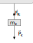
\includegraphics[width=0.2\textwidth]{fili_01_01.pdf}
\end{figure}

Sul corpo agiscono due forze.
\begin{enumerate}
\item[$\vec{P}_c$] : la forza peso del corpo stesso 
\item[$\vec{F}_{fc}$]: la forza esercitata dal filo sul corpo
\end{enumerate}

\[ \vec{F}_{tot} = \vec{P}_c+\vec{F}_{fc} \]

La fune esercita la sua forza nel punto di contatto con il corpo.

È possibile considerare il corpo come se fosse un unico punto: il centro di massa
del corpo, dove agiscono tutte le forze.

Il corpo è a riposo quindi la forza totale che agisce su esso è nulla: 
\[ \vec{f}_{tot} = 0 N \]
Ne consegue che:
\[  \vec{P}_c = -\vec{F}_{fc} \]
\[ | \vec{P}_c | =  |\vec{F}_{fc} | = m_cg =7kg\cdot 9.81 \frac{m}{s^2} = 69N \]

Terzo principio della dinamica: la forza $\vec{F}_{fc}$ esercitata dal filo sul 
corpo è uguale e contraria alla forza $\vec{F}_{cf}$, esercitata dal corpo sul filo
,che è la grandezza da trovare.

\begin{figure}[h]
\centering
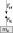
\includegraphics[width=0.1\textwidth]{fili_01_02.pdf}
\end{figure}

\[ \vec{F}_{cf} = - \vec{F}_{fc} \]
\[ | \vec{F}_{cf} | = | \vec{F}_{fc} | = 69 N \]

Il soffitto, anch’esso in quiete, esercita una forza $\vec{F}_{sf}$
uguale e contraria alla forza $\vec{F}_{fs}$ che il filo esercita sul soffitto.

\begin{figure}[h]
\centering
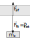
\includegraphics[width=0.2\textwidth]{fili_01_03.pdf}
\end{figure}

Questa forza $\vec{F}_{fs}$ è uguale alla forza $\vec{P}_{tot}$
determinata dal peso del corpo e del filo, ma con un punto di applicazione
diverso.
\[ - \vec{F}_{sf} = \vec{F}_{fs} = \vec{P}_{tot} \]
\[ \vec{P}_{tot} = \vec{P}_c + \vec{P}_f \]
\[ |\vec{F}_{sf}| = |\vec{P}_{tot} = | \vec{P}_c | + | \vec{P}_f  | = m_cg+m_fg= \]
\[ (7 kg + 50 g) \cdot 9.81 \frac{m}{s^2} = (7 kg + 0,05 Kg) \cdot 9.81 \frac{m}{s^2}
= 69.2 N \]


